\documentclass[12pt, letterpaper]{article}
\usepackage[utf8]{inputenc}
\usepackage[english]{babel}
\usepackage{fancyhdr}
\usepackage{geometry}
\usepackage{natbib}
\bibliographystyle{besjournals}
%\addbibresource{references.bib}
\newcommand{\pkg}[1]{{\fontseries{b}\selectfont #1}}
\usepackage{booktabs, tabularx, longtable}
\usepackage{array}
\usepackage{colortbl}
\usepackage{graphicx}
\usepackage[section]{placeins}
\usepackage{amsmath}
\usepackage[leftcaption]{sidecap}
\graphicspath{ {./figures/} }
\usepackage{setspace}
\usepackage{caption}
\captionsetup[table]{font={stretch=1.05, small}}     %% change table caption spacing
\captionsetup[figure]{font={stretch=1.05, footnotesize}} %% change figure caption spacing
\usepackage{titlesec}
\titleformat{\section}
  {\normalfont\fontsize{14}{15}\bfseries}{\thesection}{1em}{} %change the size of section header font
\titleformat{\subsection}
  {\normalfont\fontsize{12}{15}\bfseries}{\thesubsection}{1em}{} %change the size of subsection header font
\renewcommand{\thesection}{}  %remove the section numbers
\renewcommand{\thesubsection}{} %remove subsection numbers

%try to deal with the problem of too long figure caption
\DeclareCaptionLabelFormat{adja-page}{\hrulefill\\#1 #2 \emph{(previous page)}}
\usepackage{subfig}

%try to deal with issue of figures going to the end of the document
\makeatletter
\AtBeginDocument{%
  \expandafter\renewcommand\expandafter\subsection\expandafter{%
    \expandafter\@fb@secFB\subsection
  }
}
\makeatother

\geometry{margin = 1in}
\pagestyle{fancy}
\fancyhf{}
%set the header
\rhead{\thepage}
\lhead{A.Stears}
%set the line spacing
\renewcommand{\baselinestretch}{2}
%add line numbers
\usepackage{lineno}
\linenumbers


%\title{Demographic trade-offs affect how leaf turgor loss point and tissue dry matter content mediate the effect of drought on herbaceous perennial survival and growth} 
%\author[1]{Alice Stears}
%\author[2]{Peter Adler}
%\author[3]{Dana Blumenthal} %ask Dana if there are any additional authors we should include-- i.e. Kevin Mueller?
%\author[3]{Julie Kray}A demographic trade-off determines how Leaf turgor loss point and tissue dry matter content mediate the effect of drought on herbaceous perennial survival and growth
%\author[4]{Troy Ocheltree}
%\author[5]{Kevin Wilcox}
%\author[1]{Daniel C. Laughlin}

% Include full affiliation details for all authors
%\affil[1]{Botany Department and Program in Ecology, University of Wyoming, Laramie, WY}
%\affil[2]{Department of Wildland Resources and the Ecology Center, Utah State University, Logan, UT}
%\affil[3]{USDA-ARS Rangeland Resources Research Unit, Fort Collins, CO}
%\affil[5]{Department of Ecosystem Science and Management, University of Wyoming, Laramie, WY}
%\affil[4]{Warner College of Natural Resources, Colorado State University, Fort Collins, CO}

\begin{document}

\begin{flushleft}
\Large{\textbf{Demographic trade-offs affect how leaf turgor loss point and tissue dry matter content mediate the effect of drought on herbaceous perennial survival and growth}} 

\normalsize{Alice E. Stears$^{1*}$, Peter B. Adler$^2$, Dana M. Blumenthal$^3$, Julie A. Kray$^4$, Troy W. Ocheltree$^5$, Kevin R. Wilcox$^5$, Daniel C. Laughlin$^1$}

\small{$^1$Botany Department and Program in Ecology, University of Wyoming, Laramie, WY; $^2$Department of Wildland Resources and the Ecology Center, Utah State University, Logan, UT; $^3$USDA-ARS Rangeland Resources Research Unit, Fort Collins, CO, $^4$Warner College of Natural Resources, Colorado State University, Fort Collins, CO, $^5$Department of Ecosystem Science and Management, University of Wyoming, Laramie, WY}

\small{$^*$Corresponding Author: astears@uwyo.edu}

\end{flushleft}
\textbf{Keywords:} demographic rates, drought, functional traits, global change, grasslands, vital rates

\begin{abstract}
\begin{enumerate}
\item Global climate change increases the likelihood of extreme weather events and exacerbates variability in inter-annual climate, which in turn impacts plant population dynamics and community composition. Understanding how plant traits mediate individual-level demographic responses to fluctuating abiotic conditions may provide a mechanistic explanation of species responses to drought. 
%Previous work has characterized broad relationships between plant traits and regional climate, but has largely ignored how traits mediate the effect of abiotic conditions on demographic rates. Mechanistic predictions of plant community structure and function depend on understanding demographic responses to fluctuating abiotic conditions. Here we quantify the importance of leaf and root functional traits for predicting species growth and survival in response to drought, which provides insight into drought tolerance mechanisms and refines our ability to predict population and community responses to changing climate.
\item We predicted that species with low leaf turgor loss point (TLP) and higher leaf and root dry matter content (LDMC and RDMC) are more likely to survive and grow in dry years because plants with higher rates of carbon allocation to cell walls and an ability to chemically maintain osmotic pressure in leaf cells will have higher wilting resistance. We predicted that these traits will not impact growth and survival in wet years when plants are not drought stressed. 
\item We synthesized 15 years of demographic data, species-level  functional trait measurements, and records of annual climate in a short-grass steppe ecosystem in northern Colorado (COSGS). We calculated the Standardized Precipitation Evapotranspiration Index (SPEI) for each growing season as a measure of drought intensity. We fit Generalized Linear Mixed Effect Models to determine whether traits interact with drought intensity to impact growth and survival while accounting for plant size and local intraspecific competition. 
\item  Plant size had consistently positive effects on survival across all species. Local intraspecific competition had consistently negative effects on growth and survival across all species. Graminoids with more negative leaf TLP and higher LDMC and RDMC had higher survival rates in dry years, while graminoids with less negative leaf TLP and lower LDMC and RDMC had higher survival rates in wet years. Graminoids with more negative leaf TLP and higher LDMC had slower growth rates in dry years, while graminoids with less negative leaf TLP and lower LDMC had higher growth rates in wet years. Forbs demonstrated similar yet more variable responses to inter-annual climate. 
%TLP, LDMC, and RDMC interact significantly with SPEI to predict survival probability. Individuals with more negative TLP and higher LDMC and RDMC had higher survival rates in drier years, while the opposite was true in wet years. The two morphological traits (LDMC and RDMC) had a stronger effect on survival than TLP. This contradicted our predictions, and might indicate that leaf and root structural integrity is more important than osmotic maintenance for maintaining turgid leaves under water stress. %if it's a better predictor, isn't it also more important?
\item  The  effects  of  abiotic  environmental variation  are  mediated  by  plant functional traits,  which  dictate  the  nature  of  a plant’s physiological response and the associated impact on demographic rates. Our results show that traits impact survival and growth in opposite ways, which is evidence of a trade-off between these two demographic rates. We also found that leaf TLP is a good predictor of both growth and survival in response to drought, and that LDMC and RDMC are equal or better predictors. Finally, we also identified evidence of a trade-off between competition and drought tolerance. These results advance our understanding of the mechanisms by which drought intensity drives plant population dynamics, and will refine our predictions of how plant communities will respond to more intense and frequent drought.

%make synthesis better
\item \textit{Synthesis} The  effects  of  abiotic  environmental variation  are  mediated  by  plant functional traits, which dictate the nature of a plant’s physiological response and the associated impact on demographic rates. Traits impacted survival and growth in opposite ways, illustrating the importance of accounting for demographic trade-offs when evaluative how traits effect demographic responses to environmental change. The physiological trait leaf TLP is a good predictor of both growth and survival in response to drought, but the easier-to-measure morphological traits LDMC and RDMC are equal or better predictors. These results advance our understanding of the mechanisms by which drought intensity drives plant population dynamics, and will refine our predictions of how plant communities will respond to more intense and frequent drought.
\end{enumerate}
\end{abstract}

\section{Introduction}
As the frequency and intensity of extreme climate events increases with climate change, it becomes increasingly important to understand how plant populations and communities will respond \citep{Vicente-Serrano2020AWarming}. Climate models predict that some regions will receive more precipitation in concentrated extreme-precipitation events, while other regions will receive less moisture overall with longer periods of more extreme drought between precipitation events \citep{Knapp2008ConsequencesEcosystems}. While climate models struggle to predict fine-scale variation in precipitation, it is generally agreed that western North America will undergo more frequent and intense drought as climate change progresses \citep{Hartmann2013}. The impacts of global change are primarily driven by the impacts of environmental variation on individual-level processes such as growth, reproduction, and survival.  

Previous work has characterized variation in community-level functional trait values along gradients of aridity. Both experimentally-induced and naturally-occurring gradients of water availability drive shifts in community-weighted mean (CWM) trait values for traits including specific leaf area (SLA), such that drier communities have lower CWM-SLA \citep{Nunes2017WhichDrylands,Cornwell2009CommunityCalifornia}. Other studies have identified little to no variation in CWM traits after drought, but have identified either decreased functional diversity (FD) in dry sites \citep{Luo2019LongGrasslands} or increased FD immediately after experimentally- induced drought \citep{Griffin-Nolan2019}. Additional work in North American shortgrass steppe has examined the relationship between traits and species-level responses to precipitation availability and grazing, and indicates that low leaf osmotic potential (turgor loss point), high leaf dry matter content (LDMC) and low SLA are related to decreased sensitivity to interannual precipitation variability \citep{Wilcox2020PlantPrairie}. In this same system, LDMC and senescence date are important traits for predicting species-level responses to both drought and grazing \citep{Blumenthal2020}. Determining how these traits affect growth and survival of individual plants responding to variable inter-annual climate will provide a mechanistic understanding of these patterns.

Individual-level impacts of abiotic variation are observed first in the physiological responses of plants to stress, such as wilting in response to decreased water availability \citep{Bartlett2012}. After a plant's physiological ability to withstand or escape drought is surpassed, death or decreased fecundity negatively impacts population sizes for more drought-susceptible species. Community composition is then altered, as are the competitive and facilitative interactions between individuals within that community \citep{Ploughe2019CommunityInteractions}. In extreme cases, this process can lead to either species extirpation or recruitment of formerly absent species to the local species pool, changing both the functional and phylogenetic diversity of the plant community.  Evaluating the underlying demographic mechanisms and plant-plant interactions that are driving community dynamics is an important next step in functional and population ecology in order to understand and predict how the extreme climate impacts on demographic rates are mediated by the phenotypic traits of plants \citep{Laughlin2020TheFitness,Ploughe2019CommunityInteractions,Hoover2014ResistanceExtremes,Salguero-Gomez2012}.   

In order to isolate the importance of functional traits for plant responses to drought, we must first recognize and account for factors unrelated to functional traits that impact how plants respond to abiotic conditions. First, we must account for individual plant size. An individual is more likely to survive to the next year if it is larger and more established than a smaller individual of the same species \citep{Tredennick2017}. Second, competition between individuals also negatively impacts demographic rates \citep{Adler2012}. Third, demographic rates often differ in their sensitivity to environmental variation, as well as their relative importance for whole-plant fitness \citep{Laughlin2020TheFitness,Dibner2019}. Even after accounting for these known drivers of demography, we lack a general understanding of which traits interact with drought to drive plant demographic rates, and thus fitness \citep{Laughlin2018,Laughlin2020TheFitness}(Fig.\ref{fig:ConceptFig}). Here, we identify how plant functional traits related to water use impact species growth and survival, two critical components of fitness for perennial plants, across a temporal gradient of water availability in a Colorado shortgrass steppe ecosystem. 

%While definitions of "functional traits" abound \citep{Violle2007,Volaire2020WhatProcesses,Mcgill2006}, a majority of plant functional trait-based studies focus on a similar set of traits, specifically "leaf economic traits" such as specific leaf area (SLA) \citep{Wright2004} and "root economic traits" such as root tissue density \citep{Kramer-Walter2016}. These economic traits are often morphological, and while they are indicative of different strategies to deal with stress and disturbance, they typically do not directly measure the physiological mechanisms that underpin these strategies. Because of this, some argue that these traits are most useful for predicting and identifying population or species-level responses to environmental variation, but  have limited utility when predicting how individual plants respond to variation in environmental conditions \citep{Volaire2018}. Instead, physiological traits such as cavitation resistance or osmotic potentials might be more useful for identifying patterns of individual plant responses to abiotic conditions such as soil water availability. While this dichotomy between 'functional and physiological traits' and their respective utility may be too strict, it does highlight the importance of considering plant traits that directly measure the physiological processes underlying plant adaptations to abiotic variation.

One reason functional traits such as SLA or leaf dry matter content (LDMC) are so commonly used is that they are relatively easy and fast to measure, making it practical to sample many replicates. Physiological measurements, on the other hand, are often labor intensive and impractical to assess across many individuals or species. We focus on the physiological trait leaf turgor loss point (TLP), which measures the osmotic pressure within a leaf at which cells begin to lose turgor and the leaf loses function \citep{Bartlett2012a}. Species or individuals that can withstand more water loss  before losing leaf cell turgor (have a more negative TLP) have a greater physiological drought tolerance. This trait is traditionally measured by creating pressure volume curves, a labor and time-intensive process, but recent advances have identified a method that is much faster and easier. This method uses a vapor pressure osmometer to identify the leaf osmotic potential, or leaf cell solute potential at full hydration, which is tightly correlated with with leaf TLP in woody species \citep{Bartlett2012}. Subsequent work has shown that leaf osmotic potential is also tightly linked with leaf TLP in herbaceous species in western North American grasslands, and is correlated with traits with established links to drought tolerance \citep{Griffin-Nolan2019}. TLP has been linked to leaf-level drought tolerance, since species with lower leaf TLP have the ability to maintain cell turgor, stomatal and hydraulic conductance, and gas exchange at more negative soil water potentials than species with less negative leaf TLP \citep{Bartlett2012a}. Leaf TLP is also predictive of species abundances in semiarid systems, where lower TLP species have lower precipitation sensitivity \citep{Wilcox2020PlantPrairie}. In these systems, leaf TLP is also correlated with other traits that linked herbivory resistance, drought tolerance, and resource conservative growth strategy such as high LDMC, low leaf nitrogen and phosphorous, and high stem density \citep{Blumenthal2020}. However, the extent to which TLP variation mediates the effect of drought on plant survival and growth is not known. Despite advances in methodology for TLP measurement, traits such as LDMC and root dry matter content (RDMC) are still easier to measure, and may be as good as physiological traits at predicting drought tolerance across a gradient of water availability \citep{Bartlett2012,Griffin-Nolan2019,Blumenthal2020}.

To address these knowledge gaps, we evaluated whether species-level functional trait measurements improve our predictions of plant survival probability and growth across a gradient of drought intensity. We integrated long-term demographic data from chart-quadrats, climate records, and species-level trait measurements to develop statistical models that quantify how traits predict survival and growth, and how the nature of that relationship changes according to inter-annual drought intensity. We predicted that (1) species with low TLP and high tissue DMC (dry matter content) will have higher growth and survival rates in dry years than species with high TLP and low tissue DMC (Fig.{fig:ConceptFig}). We also predict that (2) both physiological and morphological traits related to water use, such as TLP and LDMC, will be better predictors of growth and survival in response to drought when compared to leaf economic traits, such as SLA \citep{Wright2004, Reich2014}. Like SLA, LDMC is correlated with plant relative growth rate and resource-acquisition strategy \citep{Weiher1999ChallengingEcology}, but is a more direct measurement of leaf structure and allocation of carbon to leaf tissue than SLA \citep{Niinemets1999ComponentsPlants,Hodgson2011}. Species with higher LDMC have higher allocation to cell wall structure and more densely-packed leaf cells, and thus are more likely to maintain cell turgor under water stress \citep{Niinemets2001Global-scaleShrubs,Poorter2009CausesMeta-analysis,Wilcox2020PlantPrairie}. We also predict that (3) physiological traits will be stronger predictors of survival than easy-to-measure functional traits, since they are more direct measurements of physiological processes that impact growth and survival. Finally, we expect that (4) in this semiarid system, traits that are related to water use will predict growth and survival in dry years, but will not be important for predicting demographic rates in wet years when plants are not as water-limited. 

\begin{figure}
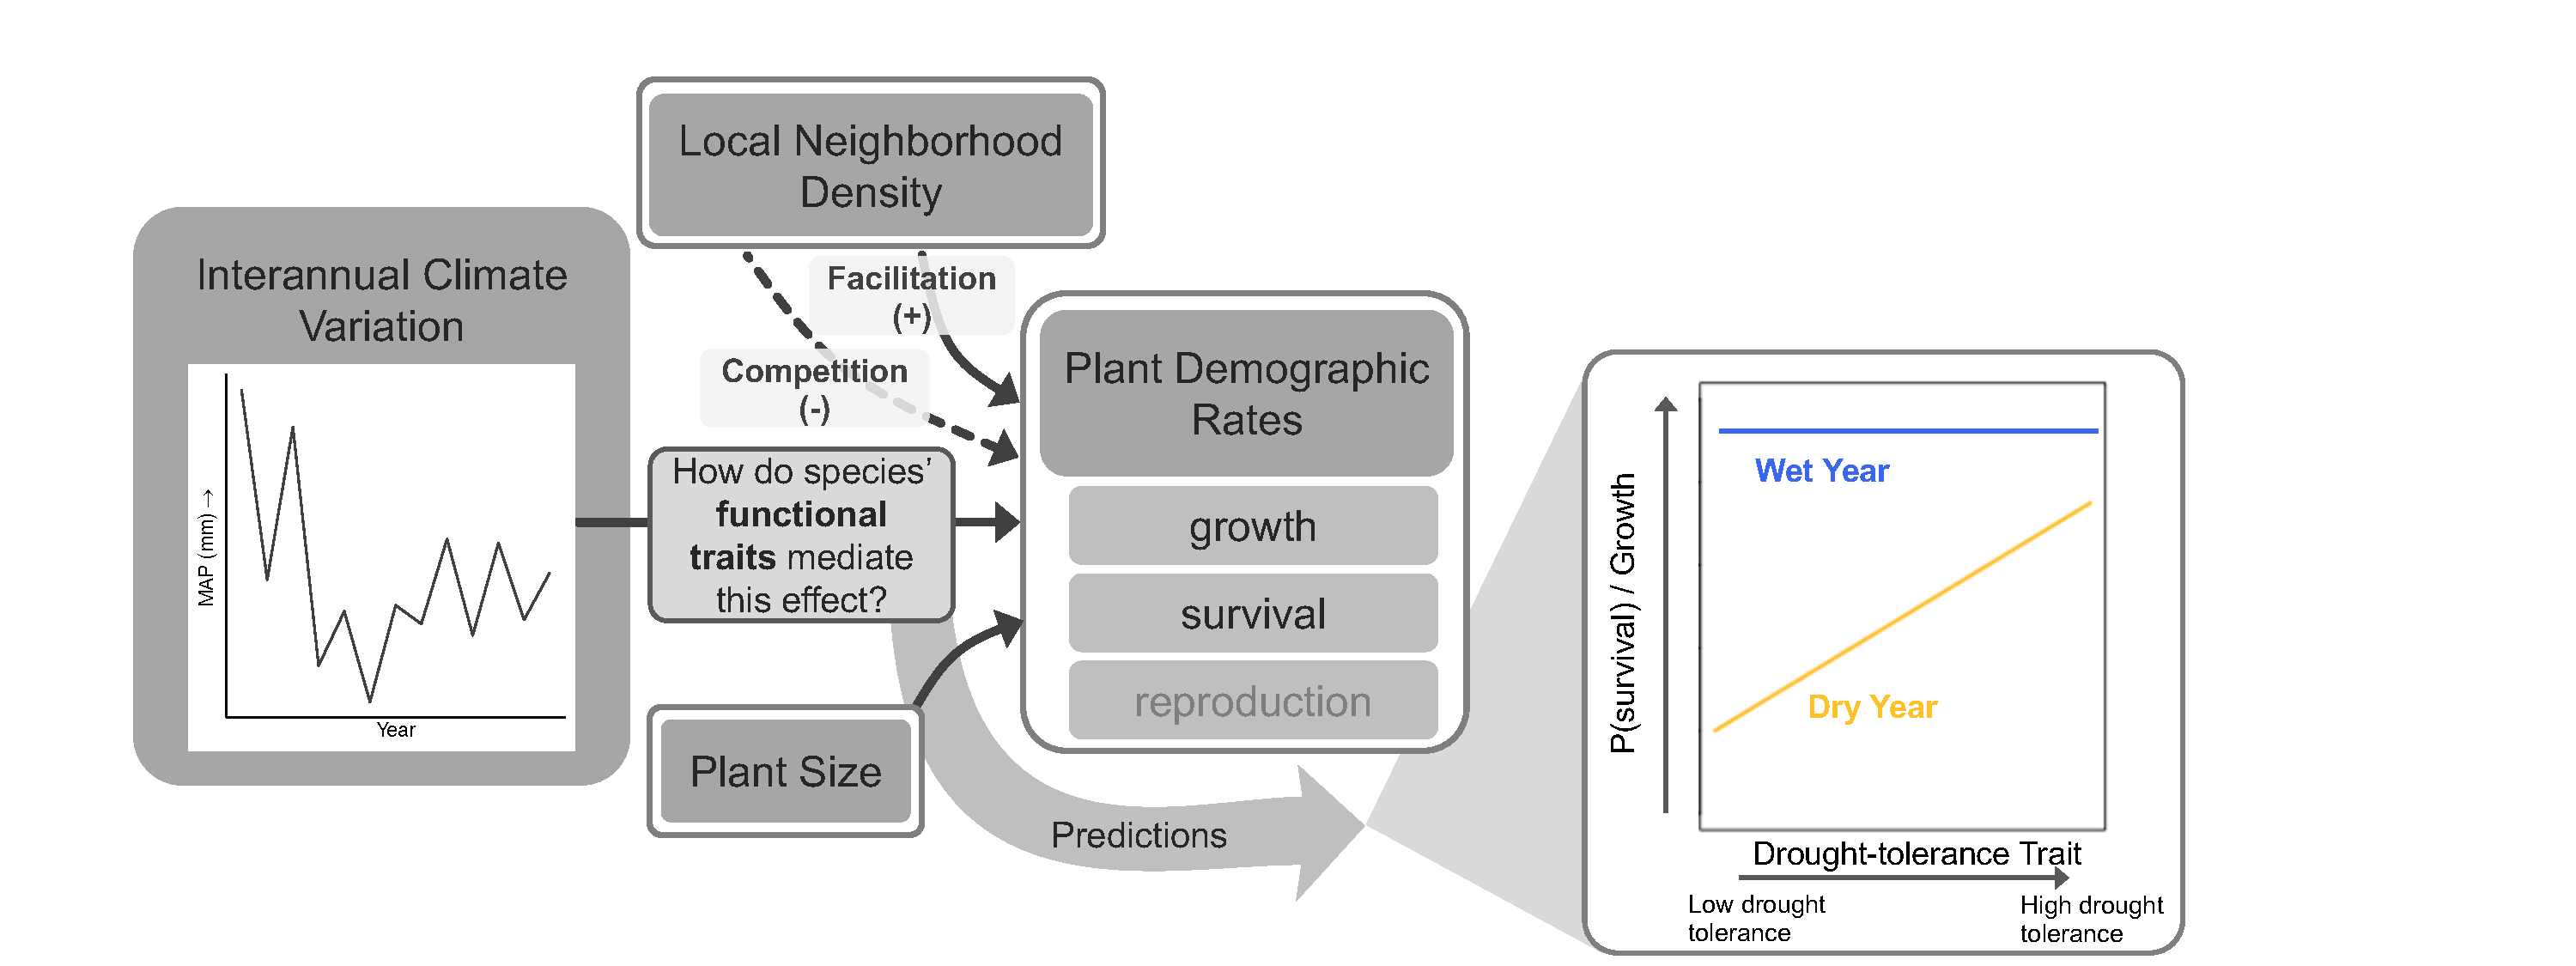
\includegraphics[width=1\textwidth]{CO_sgs_ConceptualFigure.pdf}
\caption{\small{
The demographic rates of growth, survival, and reproduction, are impacted by environmental variation, interactions with local neighbors, and plant size. We focus here on plant growth and survival given a lack of information of recruitment rates. The impact of environmental variation on an organism's demographic rates is likely mediated by the functional traits of that organism. This is especially likely for traits that are related to environmental conditions that are most limiting or stress-inducing in a given habitat. For example, traits related to water use might be more important for plant growth and survival in very dry years, and relatively less important in years with high water availability. The figure on the right of this diagram shows how a trait related to drought-tolerance may mediate the effect of climate on growth and survival. Specifically, we predicted that traits impact survival or growth rates in dry years, but are not important in wet years when a plant is not experiencing severe water stress. 
}}
\label{fig:ConceptFig}
\end{figure}

\section{Methods}
\subsection{\textit{Demographic Data}} We monitored growth and survival for eight graminoid and eight forb species for 13 continuous annual transitions over 24, 1-m$^2$ chart-quadrats at the Central Plains Experimental Research Location (CPER) in Nunn, Colorado, USA (40.8$^o$N/110.8$^o$W). These quadrats were established as part of the Shortgrass Steppe Long Term Ecological Research project \citep{Chu2013}. This site is located at 1650 m elevation in the North American shortgrass steppe, which is dominated by \textit{Bouteloua gracilis} and \textit{Bouteloua dactyloides}. It receives an average of 340 mm of precipitation annually, and has a mean annual temperature of 8 $^o$C \citep{Chu2014}. Soils at the CPER are primarily Mollisols and Aridisols.

The chart-quadrat method used does not assign each individual a unique identifying number or tag, but does map each individual plant in a spatially explicit manner each year. Bunchgrasses, shrubs, and other plants with a sizeable basal area were mapped as polygons, while grasses and forbs with a small number of stems were mapped as points. Of the species included in this analysis, graminoids were measured as polygons, and forbs were measured as points, so each data type will be referenced as either "graminoids" or "forbs," respectively.  Growth can only be extracted from this dataset for individuals measured as polygons, because size is not measured for points. We calculated growth as log(size$_{t+1}$/size$_t$) for each individual.  

We extracted growth and survival data from a digitized version of this map dataset using "tracking algorithms" in R \citep{Lauenroth2008, RCoreTeam2019}. These algorithms loop through the annual maps for a given quadrat, and assume that individuals of the same species growing in the same location in consecutive years are the same individual. In this way, the algorithms generate records of survival for all individuals, and records of growth or shrinkage for individuals measured as polygons. Individual plants can go dormant for up to several years, such that no above-ground material is visible. These tracking scripts allow for a user-defined period of dormancy, which we set to the conservative limit of one year. This means that if an individual is present in year 1, absent from the maps in year 2, but present in year 3 at the same coordinates as year 1, this plant is considered to be the same individual. We also allow a 'buffer' of 5 cm in observations of the same individual from year to year, which accounts for measurement error as well as true variation in re-sprouting location across years. 
\subsection{\textit{Climate Data}} The standardized precipitation-evapotranspiration index (SPEI) is a metric of drought intensity that uses temperature and precipitation data to estimate evapotranspiration \citep{Vicente-Serrano2010}.  To calculate SPEI for this analysis we used climate data from the Global SPEI database, which calculates SPEI at a 55 $km^2$ resolution \citep{Vicente-Serrano2010}. SPEI can be calculated over an interval as short as one month, or as long as 48 months. In this study, each species has a unique phenology and potentially reacts to timing of drought differently. Therefore, we calculated SPEI for each species using an SPEI interval that matches their growth phenology. For example, for a species that grows and flowers from May through August, SPEI is calculated each year with a four month interval that ends in August. The beginning of the growth interval was assumed to be one month before the start of flowering (This is illustrated in Fig.\ref{fig:SPEI_fig}). Flowering phenology intervals were collected from a Colorado flora \citep{Ackerfield2015}.  
\subsection{\textit{Trait Data}} We measured leaf and root functional traits for the graminoid, shrub, and forb species that comprise most of the diversity in the demographic dataset. Five to ten mature and healthy individuals of each target species were collected for each target species. A majority of the trait values used in this analysis come from samples collected at the USDA-ARS CPER. Several other species were measured at USDA-ARS High Plains Grasslands Research Station (HPGRS) near Cheyenne, WY, a northern mixed-grass prairie within 35 miles of the CPER. Samples for trait measurement were collected at CPER and HPGRS between 2014 and 2018 \citep{Blumenthal2020}. We supplemented this dataset with leaf and root trait data measured from samples collected at the University Pasture in Hays, KS (southern mixed-grass prairie), the USDA-ARS Ft. Keogh Livestock and Range Research Station in Miles City, MT (northern mixed-grass prairie), and the USDA-ARS US Sheep Experiment Station near Dubois, ID (sagebrush steppe). See (Table S \ref{TraitMeasurements}) for a list of sampling locations for each species included in this analysis. 

We measured species-level average trait values for seven traits: specific leaf area (SLA; cm$^2$/g), leaf dry matter content (LDMC; g/g), turgor loss point (TLP; MPa), specific root length (SRL; g/m), average root diameter (RDiam; mm), root dry matter content (RDMC; g/g), and root tissue density (RTD; g/cm$^3$). SLA and LDMC were measured using standard methods \citep{Perez-Harguindeguy2013}. TLP was calculated from measurements of leaf osmotic potential made using a Vapro 5600 osmometer \citep{Bartlett2012, Griffin-Nolan2019}. TLP was derived from osmotic potential using the following equation: leaf turgor loss point $= 0.944($leaf osmotic potential$) - 0.611$. Below ground traits were measured for fine, absorptive root tissue (typically 1st-3rd order roots) \citep{McCormack2015}. Root length, average diameter, and root volume were measured using WinRhizo software. Further details of leaf and root trait sampling and measurement protocols can be found in \cite{Blumenthal2020}.

\subsection{\textit{Statistical Analysis}} We use a generalized linear mixed model (GLMM) framework to identify how the effect of trait values on growth and survival varies across a spectrum of drought intensity. We also use this model framework to assess the relative ability of each trait to predict growth and survival. We used the lme4 package in R to fit GLMMs with a binomial error distribution and a logit link function, as well as random effects for species, quadrat, year, and plant size, to quantify the interactive effects of climate and trait values on survival and growth \citep{RCoreTeam2019, Bates2015}. Individual size is an important covariate in these models, but is only available for graminoids because forbs were mapped as points in this dataset. Because of this, we modeled graminoid and forb survival separately, and forb models do not contain a size covariate or a random slope for size. We modeled the interactive effect of climate and traits on growth using a similar model framework to the one used for survival, but with a Gaussian error distribution. Growth models were only constructed for graminoids, since we do not have growth information for forbs. The global model structure for growth and survival of graminoids and forbs followed these general forms:

\begin{multline}
\label{surv_eq}
logit(survival_{t+1})\sim \alpha + \gamma_{species}+ \delta_{quad} + \tau_{year} + size_t(\beta_{species}  + \beta_1) + trait\beta_2+ SPEI\beta_3\\ + nearEdge\beta_4  + neighborhoodDensity\beta_5 + trait\times SPEI\beta_6
\end{multline}
\begin{multline}
\label{grow_eq} 
ln(\frac{size_{t+1}} { size_{t}} )\sim \alpha + \gamma_{species}+ \delta_{quad} + \tau_{year} +   trait\beta_1+ SPEI\beta_2\\ + nearEdge\beta_3  + neighborhoodDensity\beta_4 + trait\times SPEI\beta_5
\end{multline}
Survival models use a binary response variable indicating whether an individual survived (1) or died (0) in year \textit{t+1}. The response variable for growth models is the log of the ratio of plant size in year \textit{t+1} and year \textit{t} \citep{Dalgleish2011ClimatePlants, Dahlgren2009LinkingHerb}. In both model frameworks, the fixed effects of interest are SPEI, trait, and the SPEI-by-trait interaction. We created separate growth and survival models for each trait, since we are interested in the relative ability of each trait to predict drought tolerance along a gradient of SPEI. To account for the effects of individual plant size \citep{Tredennick2018} and competition on demographic rates (Fig.\ref{fig:ConceptFig}), we included individual plant basal area (when available) and conspecific local neighborhood density as fixed effect covariates in our survival models (Equation \ref{surv_eq}). We did not include individual plant basal area as a fixed effect in models of growth, because it is already included in the denominator of the response variable, and therefore it is mathematically related to it (Equation \ref{grow_eq}).

Local neighborhood density was calculated for each individual observation, and accounts for the effect of intra-specific competition or facilitation on demographic rates, is a value we calculated for each individual observation. For graminoids, the local neighborhood density is the total plant basal area within a 10 cm radius of the focal individual that is occupied by individuals of the same species (conspecifics). For forbs, this value is a sum of the total number of conspecific stems within a 10 cm local neighborhood radius of the focal individual. We chose to calculate only intra-specific competition estimates, since it has been shown that inter-specific competition is typically weaker than intra-specific competition in dry grassland systems \citep{Adler2018,Laughlin2018}.  We tested different neighborhood radii (5, 10, 15, and 20 cm) to determine which radius is the most appropriate to use in this ecological context by fitting four generalized linear mixed-effect models for the effect of a trait-by-environment interaction on survival (following the framework of Equation \ref{surv_eq}) while including a competition metric using a different radius in each model. We compared the size of the coefficient for the fixed effect of competition in each model, and determined that the competition metric using a 10 cm radius was most appropriate because it was the largest.  We also included a fixed effect, "nearEdge," which is a binary variable indicating whether an individual was growing within 5 cm of the quadrat edge. This covariate accounts for the higher probability of 'missing' an edge individual during mapping, as well as potential under-estimation of local neighborhood density or individual size due to proximity to the quadrat edge. 

Growth and survival models for both graminoids and forbs included a random intercept for quadrat to account for spatial autocorrelation, and a random intercept for year to account for temporal autocorrelation. Because data on individual size was available for graminoids, we included a random slope for size associated with a random intercept for species, which accounts for the fact that larger individuals of a given species have a higher growth and survival probability than small individuals, but also allows for variation in response for each species. We did not include a random slope for size according to species for RTD and SRL survival models and all growth models, since model fit was singular when this random slope was included \citep{Bates2015}. Because individual size data was not available for forbs, we did not include a random slope for size in the forb survival models, but still included a random intercept for species to account for variation in trait-by-SPEI relationships across species.

We used AIC model selection to determine the best random effect structure for each model, and AIC model selection to determine the best fixed effect structure. We use the size and significance of the trait-by-SPEI interaction coefficient to rank traits by their respective ability to predict drought tolerance. However, we also used AIC to compare each model to a model of the same structure, but without the trait and trait-by-environment interaction coefficients (recorded as $\Delta$ AIC in Table \ref{ModResults}). This comparison indicates the extent to which traits improve the models. The larger the decrease in AIC in the trait model relative to the no-trait model, the more support for the ability of that trait to predict survival or growth in response to drought. Positive $\Delta$ AIC values indicate that including a trait improves model fit, while negative $\Delta$ AIC values indicate that including a trait did not improve model fit.

\section{Results}
\subsection{\textit{Graminoid Survival}} We detected significant positive main effects of individual plant size and significant negative main effects of local neighborhood conspecific density on survival probability across all trait models (Table \ref{ModResults}; Figure \ref{fig:Effects_Survival}). In other words, larger plants were more likely to survive than smaller plants of the same species, and individuals that share their immediate local environment with more individuals of the same species were less likely to survive. There was also a significant positive main effect of SPEI on survival probability, meaning that all plants had a higher survival probability when more water was available. In most cases, except for LDMC and RTD, the main effects of traits by themselves had no direct effect on survival and their effects were only manifested through interactions with climate. These effects explained between 32 and 58\% of the variation in survival rates (Table \ref{ModResults}). 

Models of survival for graminoids indicated that every trait except for SRL, interacted with SPEI to impact survival (Table \ref{ModResults}). The traits with the largest interaction coefficients were LDMC ($\beta _6=$-0.139,  \textit{P} $<$0.01), RDMC ($\beta _6=$-0.114,  \textit{P} $<$0.01), and TLP ($\beta _6=$0.082,  \textit{P} $<$0.01)(Table \ref{ModResults}; Fig.\ref{fig:PredsObs}). These interactions are illustrated in Fig.\ref{fig:PredsObs} \textbf{A},\textbf{D}, \textbf{G}, \textbf{J} and \textbf{M}. In dry years, survival was higher for species with lower leaf TLP and species with higher LDMC and RDMC. There was higher survival across all species in wet years, although survival was slightly lower for those species with low leaf TLP, high LDMC and RDMC. $\Delta$ AIC values indicate that LDMC, RDMC, and TLP are the traits that best predict how survival probability changes across a gradient of SPEI (Table \ref{ModResults}). 

\subsection{\textit{Graminoid Growth}} Models of graminoid growth show that in the context of drought intensity, several traits had an opposite effect on growth than they did on survival. Models of plant growth identified a significant interaction between TLP and SPEI ($\beta _5=$-0.065,  \textit{P} $<0.01$), LDMC and SPEI ($\beta _5=$0.083,  \textit{P} $<0.01$), and SLA and SPEI ($\beta _5=$0.033,  \textit{P} $<0.05$) (Table\ref{growth_ModResults}, Fig.\ref{fig:PredsObs} \textbf{B}, \textbf{E}, \textbf{H}, \textbf{K}, \textbf{N}). In dry years, species with high TLP, low LDMC, and low SLA grow more (or shrink less) than species with low TLP, high LDMC, high root diameter and high SLA. Growth is not unilaterally higher in wet years. Species with low TLP and high LDMC, root diameter and SLA are more likely to grow in wet years than they are in in dry years. But species with high TLP and low LDMC and RDMC actually are less likely to grow in wet years than they are in dry years. 

These interaction effects are the inverse of the interaction effects of SPEI and trait on survival for both graminoids and forbs (Table \ref{ModResults}, Table \ref{ForbSurv_ModResults}). While low TLP and high LDMC species have a higher survival probability in dry years, these same low TLP and high LDMC species are less likely to grow in dry years. $\Delta$ AIC values indicated that including a trait and trait-by-SPEI interaction improved model fit for models using TLP ($\Delta$ AIC = 5.18) and LDMC ($\Delta$ AIC = 3.98) (Table \ref{growth_ModResults}). There was not a significant main effect of traits alone on growth in any model, indicating that trait effects on growth are mediated through how they interact with annual climate. However, these models only explained 5-6\% of the variation in growth rates (Table \ref{growth_ModResults}). TLP and LDMC have significant interactive effects on survival and growth and improve model AIC for models of both graminoid survival and growth. However, RDMC explains survival probability for graminoids, but is not predictive of growth. SLA is an important predictor of graminoid growth, but not survival. 

 Across all models of plant growth, there was a significant negative main effect of local neighborhood conspecific density (\textit{P} $<0.01$)(Table \ref{growth_ModResults}). There was also a significant negative main effect (\textit{P} $<0.01$) of SPEI on growth for models that included TLP, LDMC, SLA, and RDMC. The negative effects of SPEI and local neighborhood conspecific density are consistent with those observed in survival models for forbs and graminoids.

\subsection{\textit{Forb Survival}} There was a negative main effect of local neighborhood conspecific density for all models of forb survival, and a significant main effect of neighborhood density in models that included TLP, LDMC, SLA, and RDMC (Table \ref{ForbSurv_ModResults}). There was not a significant effect of either SPEI or trait alone on forb survival probability. The marginal R$^2$ values are much smaller for forb models than graminoid models (all $<0.1$);  conditional R$^2$ values range from 0.4 to 0.6 (Table \ref{ForbSurv_ModResults}).

Models of plant survival for forbs indicate that LDMC ($\beta_6=$-0.338,  \textit{P} $<$0.01), RDMC ($\beta _6=$-0.304,  \textit{P} $<$0.01), and TLP ($\beta _6=$0.289,  \textit{P} $<$0.05) interacted significantly with SPEI to impact survival (Table \ref{ForbSurv_ModResults}). These interactions are displayed in Fig.\ref{fig:PredsObs} \textbf{C},\textbf{F}, \textbf{I}, \textbf{L}and \textbf{O}. In dry years, survival was higher for species with lower leaf TLP and species with high LDMC and RDMC. There was higher survival in wet years for species with high TLP and low LDMC and RDMC; however species with low TLP and high LDMC and RDMC had lower survival probability in wet years than in dry years. The  uncertainty in these estimates were much larger for forb survival models than graminoid models, as illustrated by the 95\% confidence intervals (Fig.\ref{fig:PredsObs}; Fig.\ref{fig:GramSurv_all}). $\Delta$ AIC values were highest for models using LDMC, RDMC, and TLP, which indicated that including coefficients for trait and trait-by-SPEI interaction for those traits improves our ability to predict how survival probability changes across a gradient of SPEI (Table \ref{ForbSurv_ModResults}). 

\begin{table}[h] \centering 
  \caption{Graminoid Survival Model Coefficients} 
  \label{ModResults} 
  \resizebox{\textwidth}{!}{%
\begin{tabular}{lccccccc} 
\\[-1.8ex]\hline 
\hline \\[-1.8ex] 
 & \multicolumn{7}{c}{\textit{Trait Model}} \\ 
\cline{2-8} 
\\
\\[-1.8ex] & TLP & LDMC & SLA & RDMC & RTD & SRL & RDiam\\ 
\hline \\[-1.8ex] 
 \rowcolor[gray]{.95}size_t & 2.194$^{***}$ & 2.166$^{***}$ & 2.205$^{***}$ & 1.788$^{***}$ & 2.766$^{***}$ & 2.762$^{***}$ & 2.010$^{***}$  \\
 neighbors\_10 & $-$0.602$^{***}$ & $-$0.605$^{***}$ & $-$0.597$^{***}$ & $-$0.601$^{***}$ & $-$0.427$^{***}$ & $-$0.422$^{***}$ & $-$0.580$^{***}$ \\
\rowcolor[gray]{.95}nearEdge & 0.006 & 0.005 & 0.008 & 0.002 & 0.086$^{*}$ & 0.089$^{*}$ & 0.023  \\ 
 \textbf{SPEI:trait} & 0.082$^{***}$ & $-$0.139$^{***}$ & $-$0.071$^{***}$ & $-$ 0.114$^{***}$ & $-$0.063$^{**}$ & $-$0.010 & $-$0.076$^{***}$ \\ 
 \rowcolor[gray]{.95}SPEI & 0.354$^{***}$ & 0.238$^{***}$ & 0.369$^{***}$ & 0.246$^{***}$ & 0.498$^{***}$ & 0.495$^{***}$ & 0.167$^{**}$ \\ 
 \textbf{trait} & $-$0.020 & 0.223$^{**}$ & $-$0.087 & $-$0.099 & 0.344$^{***}$ & 0.149 & $-$0.010 \\ 
 \rowcolor[gray]{.95}Intercept & $-$1.388$^{***}$ & $-$1.203$^{***}$ & $-$1.358$^{***}$ & $-$1.256$^{***}$ & $-$1.006$^{***}$ & $-$0.836$^{**}$ & $-$1.285$^{***}$ \\   \hline \\[-1.8ex] 
  $\tau_{00}$ & 0.12$_{quad}$ & 0.12$_{quad}$ & 0.12$_{quad}$ & 0.12$_{quad}$ & 0.11$_{quad}$ & 0.11$_{quad}$ & 0.12$_{quad}$ \\
  & 0.16$_{year}$ & 0.13$_{year}$ & 0.16$_{year}$ & 0.13$_{year}$ & 0.38$_{year}$ & 0.41$_{year}$ & 0.14$_{year}$ \\
  & 0.32$_{spp.}$ & 0.50$_{spp.}$ & 0.35$_{spp.}$ & 0.14$_{spp.}$ & 0.05$_{spp.}$ & 0.38$_{spp.}$ & 0.19$_{spp.}$\\
  \rowcolor[gray]{.95}$\tau_{11}$ & 1.95$_{size_t*spp}$ & 1.54$_{size_t*spp}$ & 1.98$_{size_t*spp}$ &
  0.79$_{size_t*spp}$ & & & 0.88$_{size_t*spp}$ \\
  $\rho_{01}$ & $-$0.78$_{spp.}$ & $-$0.93$_{spp.}$ & $-$0.82$_{spp.}$ & $-$ 0.48$_{spp.}$ & & & $-$ 0.67$_{spp.}$ \\
\hline \\[-1.8ex] 
\rowcolor[gray]{.95} Residual Variance & 3.29 & 3.29 & 3.29 & 3.29 & 3.29 & 3.29 & 3.29\\
n & 18,827 & 18,827 & 18,827 & 18,474 & 16,618 & 16,618 & 17,190\\ 
\rowcolor[gray]{.95} Marg./Cond. $R^2$ & 0.37/0.62 & 0.40/0.61 & 0.37/0.63 & 0.32/0.50 & 0.58/0.63 & 0.57/0.66 & 0.37/0.54 \\
AIC   & 14,832.090 & 14,807.940 & 14,835.920 & 14,804.750 & 13,315.520 & 13,326.630 & 13,532.720 \\ 
\hline 
\rowcolor[gray]{.95}$\Delta$ AIC$^\dagger$  & 15.41 & 39.57 & 11.59 & 32.57 & 9.12 & $-$1.99 & 12.33 \\
\hline 
\hline \\[-1.8ex] 
\textit{Note:}  & \multicolumn{7}{r}{$^{*}$ \textit{P} $<$0.1; $^{**}$ \textit{P} $<$0.05; $^{***}$ \textit{P} $<$0.01}\\
\multicolumn{8}{r}{$\tau_{00}$=Rand. Intercept Variance; $\tau_{01}$=Rand. Slope Variance; $\rho_{01}$=Correlation of Rand. Slope \& Intercept}\\ 
\multicolumn{8}{r}{$^\dagger$ = compares the AIC of a model with trait and trait:envi interaction as fixed effects to a model without}\\
\multicolumn{8}{r}{trait and trait:envi effects. This serves as a relative metric of the predictive power of a given trait.}
\end{tabular}} 
\end{table} 


\begin{table}[h] \centering 
  \caption{Graminoid Growth Model Results} 
  \label{growth_ModResults} 
  \resizebox{\textwidth}{!}{%
\begin{tabular}{lccccccc} 
\\[-1.8ex]\hline 
\hline \\[-1.8ex] 
 & \multicolumn{7}{c}{\textit{Trait Model}} \\ 
\cline{2-8} 
\\
\\[-1.8ex] & TLP & LDMC & SLA & RDMC & RTD & SRL & RDiam\\ 
\hline \\[-1.8ex] 
  \rowcolor[gray]{.95} neighbors\_10 & $-$0.216$^{***}$ & $-$0.213$^{***}$ & $-$0.218$^{***}$ & $-$0.217$^{***}$ & $-$0.215$^{***}$ & $-$0.215$^{***}$ & $-$0.218$^{***}$ \\
 SPEI & 0.103$^{***}$ & 0.144$^{***}$ & 0.113$^{***}$ & 0.131$^{***}$ & 0.082$^{*}$ & 0.087$^{*}$ & 0.035  \\ 
 \rowcolor[gray]{.95}\textbf{trait} & $-$0.022 & $-$0.012 & 0.041$^{*}$  &  0.017  & 0.031 & 0.040$^{*}$ & $-$0.014\\ 
  nearEdge & $-$0.115$^{***}$ & $-$0.114$^{***}$ & $-$0.117$^{***}$ & $-$0.116$^{***}$ & $-$0.118$^{***}$ & $-$0.119$^{***}$ & $-$0.119$^{***}$ \\ 
 \rowcolor[gray]{.95}\textbf{SPEI:trait} & $-$0.065$^{***}$ & 0.083$^{***}$ &  0.033$^{**}$ &  0.002  & $-$0.020 &  0.017  &  0.050$^{***}$ \\ 
 Intercept & 0.189$^{***}$ & 0.185$^{**}$ & 0.172$^{***}$ & 0.177$^{**}$ & 0.201$^{**}$ & 0.205$^{**}$ & 0.203$^{**}$  \\ 
\hline\\[-1.8ex]
  \rowcolor[gray]{.95}$\tau_{00}$ & 0.02 $_{quad}$ & 0.02  $_{quad}$ & 0.02 $_{quad}$ & 0.02  $_{quad}$ & 0.02 $_{quad}$ & 0.02 $_{quad}$ & 0.02 $_{quad}$ \\
  \rowcolor[gray]{.95}&0.03$_{year}$ & 0.02$_{year}$ & 0.03$_{year}$ &0.03$_{year}$ & 0.04$_{year}$ & 0.04$_{year}$ & 0.04$_{year}$ \\
  \rowcolor[gray]{.95}& 0.01 $_{spp.}$ & 0.01 $_{spp.}$ & 0.00 $_{spp.}$ &0.01$_{spp.}$ & 0.01$_{spp.}$ &0.01$_{spp.}$ & 0.01$_{spp.}$\\
 \hline \\[-1.8ex] 
 Residual Variance  & 1.58 & 1.58 &	1.58 & 1.58 & 1.55 & 1.55 &	1.56 \\
\rowcolor[gray]{.95} n & 9,497 & 9,497 & 9,497 & 9,497 & 8,802 & 8,802 & 9,018  \\  
 Marg./Cond. $R^2$ & 0.057/0.087 &	0.064/0.094&	0.059/0.087	&0.059/0.090&	0.054/0.094	& 0.054/0.090 &	0.049/0.089 \\
\rowcolor[gray]{.95} AIC & 31,400.690 & 31,401.890 & 31,414.370 & 31,421.270 & 28,956.930 & 28,956.210 & 29,747.430  \\  
\hline 
$\Delta$ AIC$^\dagger$  & 5.18 & 3.98 & -8.49 & -15.40 & -13.28 & -12.57 & -5.56 \\
\hline 
\hline \\[-1.8ex] 
\textit{Note:}  & \multicolumn{7}{r}{$^{*}$ \textit{P}$<$0.1; $^{**}$ \textit{P}$<$0.05; $^{***}$ \textit{P}$<$0.01} \\ 
\multicolumn{8}{r}{$\tau_{00}$=Rand. Intercept Variance}\\ 
\multicolumn{8}{r}{$^\dagger$ = compares the AIC of a model with trait and trait:envi interaction as fixed effects to a model without}\\
\multicolumn{8}{r}{trait and trait:envi effects. This serves as a relative metric of the predictive power of a given trait.}
\end{tabular}}
\end{table} 


\begin{table}[h] \centering 
  \caption{Forb Survival Model Coefficients} 
  \label{ForbSurv_ModResults} 
  \resizebox{\textwidth}{!}{%
\begin{tabular}{lccccccc} 
\\[-1.8ex]\hline 
\hline \\[-1.8ex] 
 & \multicolumn{7}{c}{\textit{Trait Model}} \\ 
\cline{2-8} 
\\
\\[-1.8ex] & TLP & LDMC & SLA & RDMC & RTD & SRL & RDiam\\ 
\hline \\[-1.8ex] 
 neighbors\_10 & $-$0.326$^{*}$ & $-$0.332$^{*}$ & $-$0.291$^{*}$ & $-$0.321$^{*}$ & $-$0.255 & $-$0.254 & $-$0.238 \\ 
 \rowcolor[gray]{.95}nearEdge & $-$0.399 & $-$0.385 & $-$0.394 & $-$0.395 & $-$0.300 & $-$0.277 & $-$0.343 \\ 
 \textbf{SPEI:trait} & 0.289$^{**}$ & $-$0.338$^{***}$ & 0.045 & $-$0.304$^{**}$ & $-$0.059 & $-$0.014  &  1.463\\ 
 \rowcolor[gray]{.95}SPEI &$-$0.090 & $-$0.012 & $-$0.148 & $-$0.089 & $-$0.217 & 0.592 & $-$0.597  \\  
  \textbf{trait} & $-$0.075 & $-$0.271 & $-$0.060 & $-$0.369 & 0.033 & $-$0.007 &  2.620\\
 \rowcolor[gray]{.95}Intercept & $-$1.086 & $-$1.284 & $-$1.079 & $-$1.326$^{*}$ & $-$0.768 & $-$1.174 & $-$1.840 \\ 
\hline \\[-1.8ex] 
  $\tau_{00}$ & 0.06$_{quad}$ & 0.05$_{quad}$ & 0.06$_{quad}$ & 0.04$_{quad}$ & 0.13$_{quad}$ & 0.16$_{quad}$ & 0.06$_{quad}$ \\
  & 0.24$_{year}$ & 0.24$_{year}$ & 0.22$_{year}$ & 0.23$_{year}$ & 0.27$_{year}$ & 0.36$_{year}$ & 0.22$_{year}$ \\
  & 2.33$_{spp.}$ & 2.30$_{spp.}$ & 2.37$_{spp.}$ & 2.27$_{spp.}$ & 2.17$_{spp.}$ & 4.93$_{spp.}$ & 2.77$_{spp.}$\\
\hline \\[-1.8ex] 
\rowcolor[gray]{.95} Residual Variance & 3.29 & 3.29 & 3.29 & 3.29 & 3.29 & 3.29 & 3.29\\
n & 567 & 567 & 567 & 567 & 456 & 482 & 524 \\ 
\rowcolor[gray]{.95} Marg./Cond. $R^2$ & 0.025/0.458&	0.043/0.464 & 0.014/0.454	& 0.042/0.459&	0.017/0.448	&0.027/0.633 &0.015/0.489\\
AIC & 690.531 & 688.529 & 696.040 & 690.146 & 604.654 & 605.833 & 672.272 \\ 
\hline 
\rowcolor[gray]{.95}$\Delta$ AIC$^\dagger$  & 1.561 & 3.563 & $-$3.947 & 1.947 & $-$3.827 & $-$1.041 & $-$3.049 \\
\hline 
\hline \\[-1.8ex] 
\textit{Note:}  & \multicolumn{7}{r}{$^{*}$ \textit{P}$<$0.1; $^{**}$ \textit{P}$<$0.05; $^{***}$ \textit{P}$<$0.01} \\ 
\multicolumn{8}{r}{$\tau_{00}$=Rand. Intercept Variance}\\ 
\multicolumn{8}{r}{$^\dagger$ = compares the AIC of a model with trait and trait:envi interaction as fixed effects to a model without}\\
\multicolumn{8}{r}{trait and trait:envi effects. This serves as a relative metric of the predictive power of a given trait.}
\end{tabular} }
\end{table} 

\begin{figure}
    \centering
    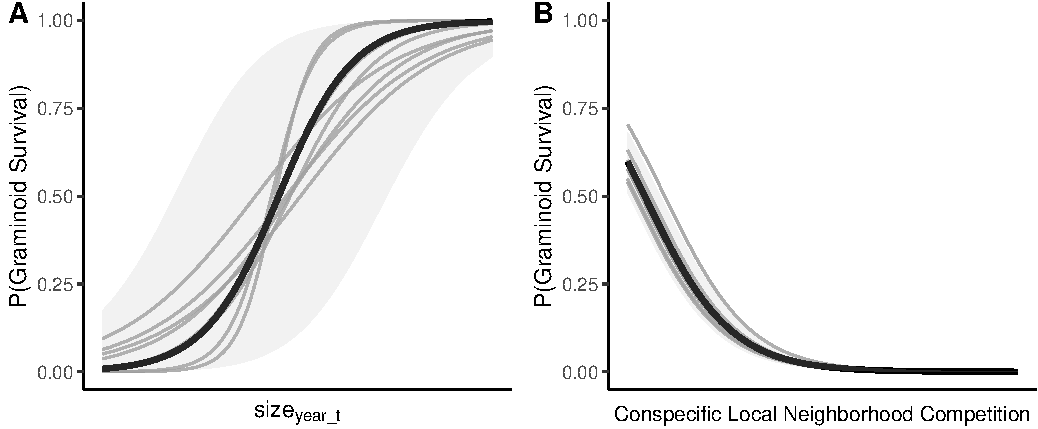
\includegraphics[width=.8\textwidth]{survEffectPlots-1.pdf}
    \caption{The effect of size in year \textit{t} (\textbf{A}) and local neighborhood density (\textbf{B}) on graminoid survival in models using LDMC as the trait predictor. For all measured graminoid species, larger individuals are more likely to survive to the next year than smaller individuals of the same species (\textbf{A}). Across all graminoid species, higher crowding of an individual's local neighborhood (10 cm radius) with individuals of the same species corresponds to lower survival probability (\textbf{B}). (\textbf{C}) shows the effect of local neighborhood density on graminoid size in year \textit{t+1} in models using TLP as the trait predictor. Across all graminoid species, higher crowding of an individual's local neighborhood (10 cm radius) with individuals of the same species corresponds to lower growth in the next year. Dark lines indicate the overall effect of each covariate on survival. The 95\% confidence interval for the overall effect of conspecific local neighborhood competition is shown in light grey. Dark grey lines indicate the effects of competition according to each species.}
    \label{fig:Effects_Survival}
\end{figure}

\begin{figure}
\captionsetup{labelformat=empty}
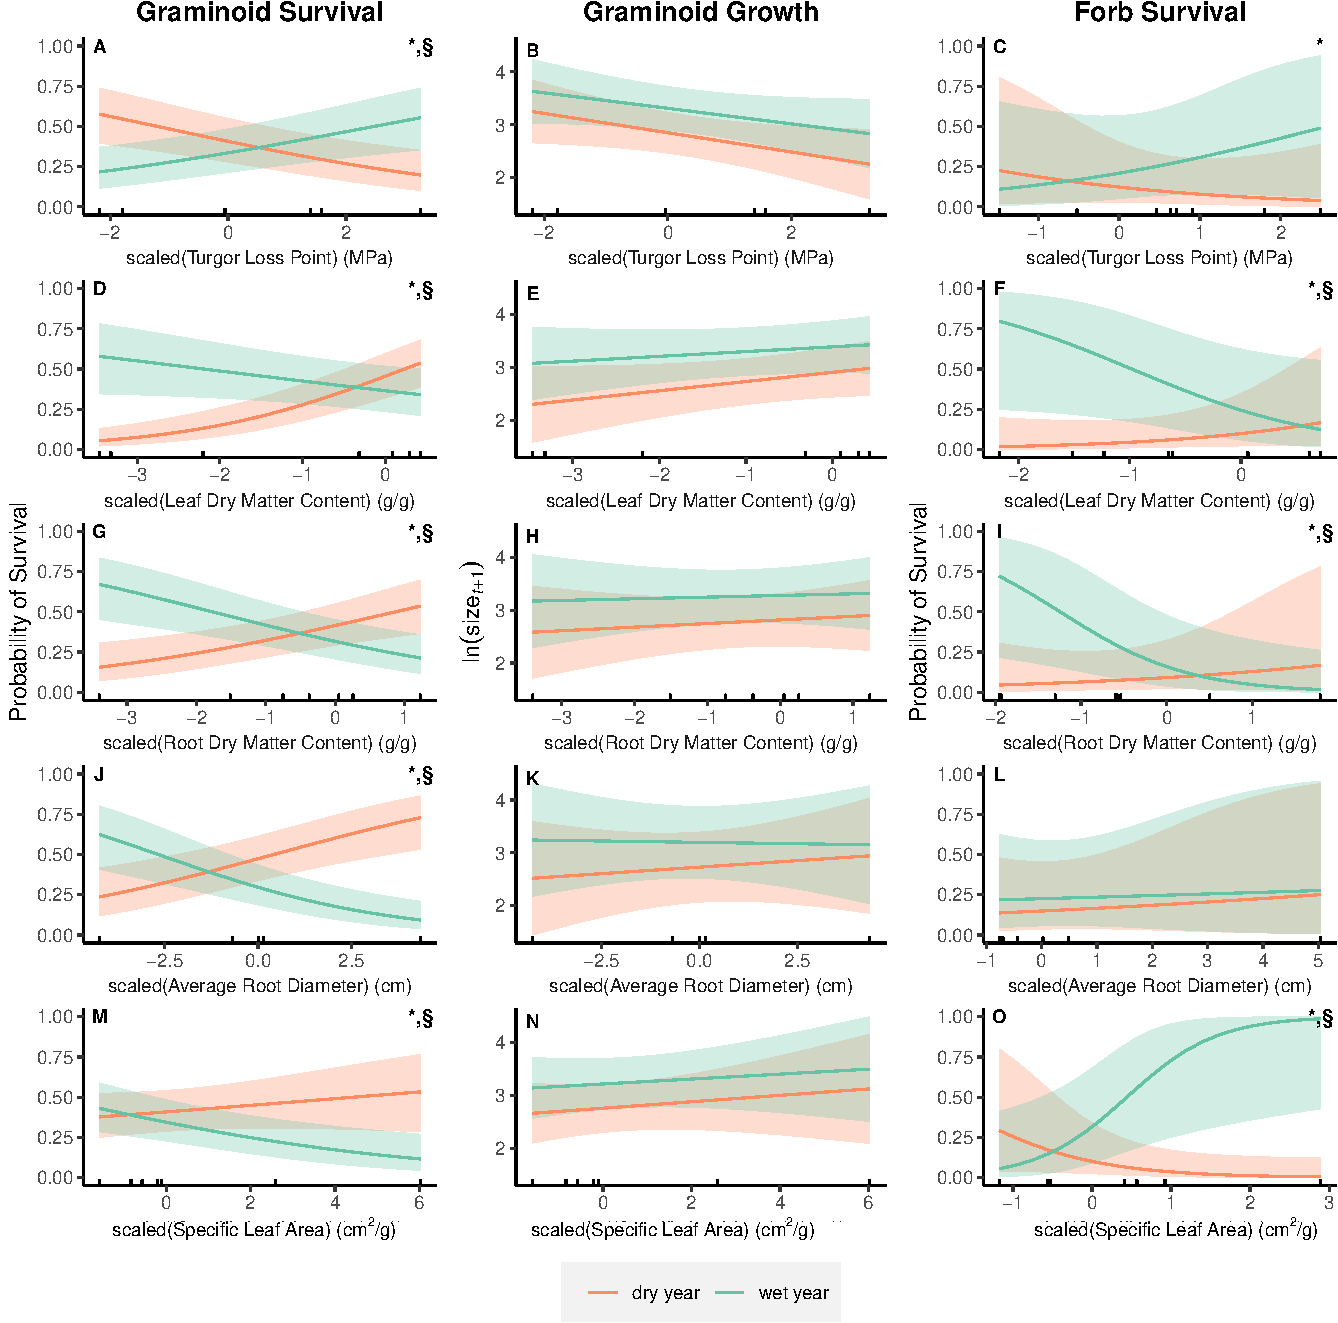
\includegraphics[width=1\textwidth]{mainObservationsFig-1.pdf}
\caption{}
\label{fig:PredsObs}
\end{figure}
\clearpage

\begin{figure}
   %\captionsetup{labelformat=adja-page}
   \ContinuedFloat
   \caption{
(\textbf{A}) Graminoid species are more likely to survive in dry years (low SPEI, orange line) if they have a low TLP than species with a high TLP, while species with a high TLP are slightly more likely to survive in wet years (high SPEI, green line) (Marg. R$^2$ = 0.37, Cond. R$^2$ = 0.62; interaction coef. = 0.08, \textit{P}$<$ 0.01). (\textbf{D}) A similar trend in graminoid survival probability is predicted by the model that includes LDMC (Marg. R$^2$ = 0.40, Cond. R$^2$ = 0.61; interaction coef. = -0.14, \textit{P}$<$ 0.01). (\textbf{G}) A similar trend to LDMC exists for graminoid survival probability as predicted by the interaction between RDMC and SPEI (Marg. R$^2$ = 0.32, Cond. R$^2$ = 0.50; interaction coef. = -0.11, \textit{P}$<$ 0.01). (\textbf{J}) There is a significant interaction between RDiam and SPEI, but including RDiam does not greatly improve model fit in comparison to a model without trait values (Marg. R$^2$ = 0.37, Cond. R$^2$ = 0.54; interaction coef. = -0.08, \textit{P}$<$ 0.01). (\textbf{M}) SLA does interact with SPEI to affect graminoid survival, but does not greatly improve model fit in comparison to a model without trait values (Marg. R$^2$ = 0.37, Cond. R$^2$ = 0.63; interaction coef. = -0.07, \textit{P}$<$ 0.01). (\textbf{B}) Low TLP graminoid species are more likely to grow in wet years (high SPEI, blue line) than in dry years (low SPEI, pink line), while high TLP species are more likely to grow in dry years than in wet years (Marg. R$^2$ = 0.06, Cond. R$^2$ = 0.09; interaction coef. = -0.07, \textit{P}$<$ 0.01). (\textbf{E}) A similar trend in graminoid growth is predicted by the model that includes LDMC (Marg. R$^2$ = 0.06, Cond. R$^2$ = 0.10; interaction coef. = 0.08, \textit{P}$<$ 0.01). (\textbf{H}) There is not a significant interactive effect of SPEI and RDMC on growth (Marg. R$^2$ = 0.06, Cond. R$^2$ = 0.10; interaction coef. = 0.002, \textit{P}$>$ 0.05) (\textbf{K}) There is a significant interaction between average RDiam and SPEI. Species with low RDiam are more likely to grow in dry years than wet years, while the opposite is true for higher RDiam species (Marg. R$^2$ = 0.05, Cond. R$^2$ = 0.09; interaction coef. = 0.05, \textit{P}$<$ 0.01). (\textbf{N}) There is also a significant interaction between SLA and SPEI. In dry years, low SLA species are more likely to grow than high SLA species, while in wet years, high SLA species are more likely to grow than low SLA species (Marg. R$^2$ = 0.06, Cond. R$^2$ = 0.09; interaction coef. = 0.03, \textit{P}$<$ 0.05). \textbf{C}, \textbf{F}, \textbf{I}, \textbf{L}, and \textbf{O} show that the trends for forb survival were similar to those observed for graminoids, although the model fit is weaker and the interaction between trait and environment is less significant for each trait (\textbf{C}: Marg. R$^2$ = 0.02, Cond. R$^2$ = 0.46; interaction coef. = 0.28, \textit{P}$<$ 0.05), (\textbf{F}: Marg. R$^2$ = 0.04, Cond. R$^2$ = 0.46; interaction coef. = -0.34, \textit{P}$<$ 0.01), (\textbf{I}: Marg. R$^2$ = 0.03, Cond. R$^2$ = 0.38; interaction coef. = -0.30, \textit{P}= 0.02), (\textbf{I}: Marg. R$^2$ = 0.04, Cond. R$^2$ = 0.46; interaction coef. = -0.30, \textit{P}$<$0.05), (\textbf{L}: Marg. R$^2$ = 0.01, Cond. R$^2$ = 0.49; interaction coef. = 1.46, \textit{P}$>$ 0.05), (\textbf{O}: Marg. R$^2$ = 0.01, Cond. R$^2$ = 0.45; interaction coef. = 0.05, \textit{P}$>$ 0.05). Black vertical bars along the x-axis (rug plots) indicate the trait values of the species included in each analysis. Survival probabilities for 'wet years' and 'dry years' are calculated for the 97.5$^{th}$ and 2.5$^{th}$ quantiles of the distribution of SPEI values. \\
* indicates that this trait-by-SPEI interaction is significant (\textit{P} $<$ 0.05)\\
§ indicates that $\Delta$ AIC for this model is positive
}
 \label{fig:test}
\end{figure}

\section{Discussion}
The demographic processes of growth, survival, and reproduction are the ultimate drivers of plant population and community dynamics, and the impact of climate change on vegetation will, at its root, be determined by the impacts of climate change on these demographic rates. However, climate change or any other variation in the abiotic environment is not acting directly on growth, survival, or reproduction. Instead, the effects of abiotic environmental variation are mediated by the functional traits of a plant, which dictate the nature of a plant's physiological response and the associated impact on demographic rates. To predict how individual plants, populations, and communities will respond to changing abiotic conditions, it is necessary to identify how functional traits mediate the abiotic effects on demographic rates. We used 15 years of demographic data, species-level trait measurements, and measurements of interannual climate variation to determine how morphological and physiological functional traits mediated the effect of drought on perennial growth and survival in a shortgrass steppe ecosystem. We found that (1) the effects of traits on survival are opposite to the effects on growth, (2) leaf TLP is an important predictor of survival probability and growth in this semiarid grassland system, (3) RDMC and LDMC are even more important than TLP for predicting survival in both graminoids and forbs, and (4) survival and growth are not uniformly higher for all species in wet years. 

 Functional traits mediate the effect of climatic variation on growth and survival in opposite ways. Species with low TLP and high LDMC are more likely to survive in dry years than species with high TLP and low LDMC, but these same drought-tolerant species are less likely to grow (Fig. \ref{fig:PredsObs}). This clearly illustrates of a trade-off between these two demographic rates \citep{Laughlin2020TheFitness}. This phenomenon, also called 'demographic compensation,' helps organisms persist in both temporally and spatially variable environments, since opposite impacts of abiotic variation on different demographic rates buffer abiotic impacts on whole-plant fitness and population growth rate ($\lambda$) \citep{Villellas2015DemographicImplications, Doak2010DemographicShifts}. A demographic trade-off in this case indicates that the functional traits that confer higher probability of survival in dry years decrease the likelihood of growing larger the next year. Such trade-offs have important implications for trait-based models of population responses, but if each of these demographic rates is impacted differently by abiotic variation, studies that only consider one of these rates will draw potentially inaccurate conclusions about how traits mediate abiotic impacts on fitness. To generate a complete picture of how traits determine plant fitness in different environments, it will be necessary to either explicitly consider growth, survival and reproduction, and quantify fitness by measuring intrinsic population growth rates \citep{Laughlin2020TheFitness}.  

 Leaf TLP, a physiological trait that measures osmotic resistance to wilting, is a good predictor of plant survival and growth in the interannually variable shortgrass steppe ecosystem (Fig. \ref{fig:PredsObs}). TLP has long been used as an indicator of physiological drought tolerance, and has been linked to drought tolerance in tropical tree species \citep{Bartlett2012}, and North American grasslands \citep{Griffin-Nolan2019, Blumenthal2020, Wilcox2020PlantPrairie}. However, our analysis represents the first test of leaf TLP to predict plant demographic responses to interannual variation in water availability. Species with a more negative leaf TLP and can lose more water before they begin to wilt and have a higher probability  of surviving in dry years than less negative TLP species. Conversely, more negative TLP species are less likely to grow in dry years than species with less negative TLP. The extent to which leaf TLP mediates demographic responses to drought needs to be tested in a greater variety of vegetation types, especially in less water-limited ecosystems to determine the role of this trait in plant drought-tolerance.   

  The morphological traits LDMC and RDMC are as good as TLP, a physiological trait, at predicting growth in response to drought, and even better than TLP at predicting survival. This contradicts the notion that physiological traits are superior tools for identifying individual responses to variation in a specific abiotic parameter \citep{Volaire2018}. This result is somewhat surprising, since TLP is a direct measure of osmotic regulation of leaf turgor and has been shown to be a good indicator of physiological drought tolerance \citep{Bartlett2012}. While LDMC and RDMC have been linked to drought tolerance, they are more indirect measurements of leaf wilting than leaf TLP, and are correlated to other functional strategies beyond drought tolerance. These results might also indicate that structural resistance to wilting is a more successful strategy in this habitat than osmotic resistance to wilting. The proportionally higher carbon investment to leaf and root structure in high LDMC and RMDC species prevents wilting and the associated loss of function, even when there is low soil water availability that might overcome osmotic wilting resistance. Although the relative importance of these traits for predicting demographic responses to drought should be tested in other systems, this result is encouraging from a methodological standpoint since LDMC and RDMC are much easier to measure than leaf TLP. 

 The interaction we identified in survival models between water-related traits and SPEI differs from our predictions. We predicted consistently high survival probability in wet years regardless of a species' position along a spectrum for any given trait. In dry years, we expected high survival for high LDMC and low TLP species and low survival for high TLP and low LDMC species (Fig.\ref{fig:ConceptFig}). The modeled survival probabilities in dry years are consistent with our expectations across the spectrum of values for TLP and LDMC. However in wet years, survival probability is not consistently high for all species. Instead, survival declines for low TLP and high LDMC species (Fig.\ref{fig:PredsObs}). This pattern could indicate a trade-off between competitive ability and drought tolerance. Species with low TLP and high LDMC are more likely to survive in dry years, but have lower survival in wet years because they are more likely to be out-competed by their neighbors with high TLP and low LDMC that are more abundant. This result contributes to a substantial body of literature that supports the existence of a trade-off between stress-tolerance and competitive ability in plant species \citep{Grime1979, Grime1997, Craine2007, Volaire2018}. 

\subsection{\textit{Synthesis}} Identifying plant traits that predict of the demographic responses to intensifying environmental stress represents a key step in formulating accurate frameworks of plant community dynamics under environmental change \citep{Laughlin2020TheFitness}. Our results challenge the notion that physiological traits are superior predictors of individual plant-level responses to abiotic conditions \citep{Volaire2018}. Specifically, we have shown that easy-to-measure morphological traits such as LDMC and RDMC explain significant variation in plant demographic responses to water stress across species in a North American grassland ecosystem. More importantly, these results advance our general understanding of the environment-dependent effect of traits on demographic rates, and reinforce the fact that different demographic rates can have divergent responses to environmental variation \citep{Laughlin2020TheFitness}. Failure to consider the consequences of demographic trade-offs will lead to inaccurate conclusions about how functional traits mediate the impacts of abiotic variation on plant fitness. 



\bibliography{references}

\renewcommand{\thetable}{S\arabic{table}} %add an "S" to the table numbers
\setcounter{table}{0} %restart table numbers at 1
\renewcommand{\thefigure}{S\arabic{figure}} %add an "S" to the figure numbers
\setcounter{figure}{0} %restart figure numbers at 1


\section{Supplementary Information}

\begin{figure}
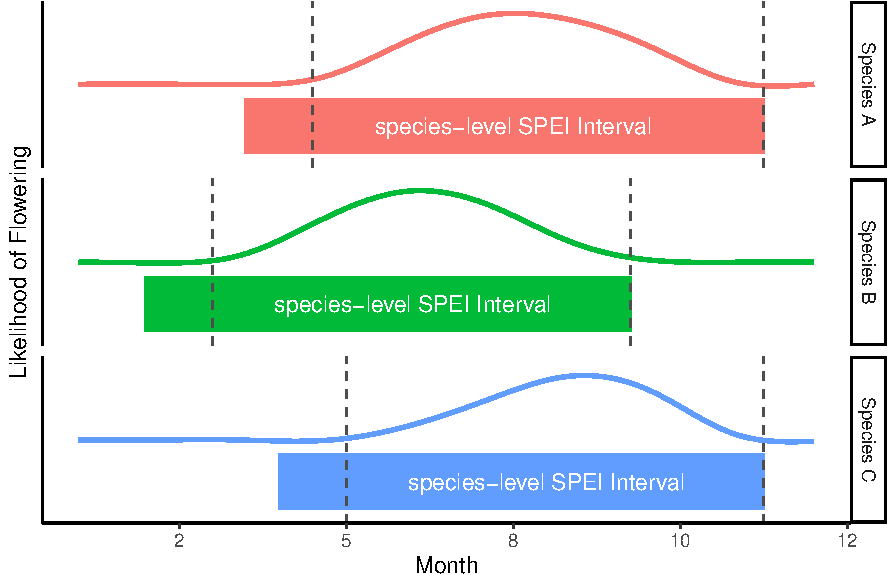
\includegraphics[width=.8\textwidth]{uniqueSPEIfig-1.pdf}
\caption{\small{
Visualization of how we calculated SPEI for each species based on its phenology. This figure shows three fictional species.
}}
\label{fig:SPEI_fig}
\end{figure}

\begin{table}[h] \centering 
  \caption{Trait Measurement Information} 
  \label{TraitMeasurements}
  \resizebox{\textwidth}{!}{%
\begin{tabular} {lccccccc|ccccc|cc} 
\\[-1.8ex]\hline 
\hline \\[-1.8ex] 
& \multicolumn{7}{c}{\textbf{Traits}} & \multicolumn{5}{c}{\textbf{Sampling Location}} & \multicolumn{2}{c}{\textbf{Func. Group}}\\
 & TLP & RootDiam & RTD & RDMC & SRL & LDMC & SLA & CPER & HPGRS & Sheep Station & Ft. Keogh  & Hays & Gram. & Forb\\ 
\hline \\[-1.8ex] 
\rowcolor[gray]{.95} \textit{Bouteloua gracilis} & $\times$ & $\times$ & $\times$ & $\times$ & $\times$ & $\times$ & $\times$ & $\times$ &&&&&$\times$&\\ 
\textit{Carex eleocharis} & $\times$ &  &  &  &  & $\times$ & $\times$ & $\times$ &&&&&$\times$&\\
\rowcolor[gray]{.95} \textit{Gaura coccinea} & $\times$ & $\times$ & $\times$ & $\times$ & $\times$ & $\times$ & $\times$ & $\times$ &&&&&&$\times$\\
\textit{Chrysopsis villosa} & $\times$ & $\times$ & $\times$ & $\times$ & $\times$ & $\times$ & $\times$ & $\times$ &&&&&&$\times$\\ 
\rowcolor[gray]{.95}\textit{Leucocrinum montanum} & $\times$ & $\times$ & $\times$ & $\times$ & $\times$ & $\times$ & $\times$ & $\times$ &&&&&&$\times$\\ 
\textit{Sphaeralcea coccinea} & $\times$ & $\times$ & $\times$ & $\times$ & $\times$ & $\times$ & $\times$ & $\times$ &&&&&&$\times$\\ 
\rowcolor[gray]{.95}\textit{Hesperostipa comata} & $\times$ &  &  & $\times$ &  & $\times$ & $\times$ & $\times$ &&$\times$&$\times$&&$\times$&\\ 
\textit{Aristida longiseta} & $\times$ & $\times$ & $\times$ & $\times$ & $\times$ & $\times$ & $\times$ & $\times$ &&&&&$\times$&\\ 
\rowcolor[gray]{.95}\textit{Bouteloua dactyloides} & $\times$ & $\times$ & $\times$ & $\times$ & $\times$ & $\times$ & $\times$ & $\times$ &&&&&$\times$&\\ 
\textit{Elymus elymoides} & $\times$ & $\times$ &  & $\times$ & & $\times$ & $\times$ & $\times$ &&$\times$&$\times$&$\times$&$\times$&\\ 
\rowcolor[gray]{.95}\textit{Sporobolus cryptandrus} & $\times$ & $\times$ & $\times$ & $\times$ & $\times$ & $\times$ & $\times$ & $\times$ &&&&&$\times$&\\ 
\textit{Thelesperma filifolium} & $\times$ & $\times$ & $\times$ & $\times$ & $\times$ & $\times$ & $\times$ & $\times$ &&&&&&$\times$\\ 
\rowcolor[gray]{.95}\textit{Allium textile} & $\times$ & $\times$ &  & $\times$ &  & $\times$ & $\times$ &  & $\times$ &$\times$&$\times$&&&$\times$\\ 
\textit{Oenothera coronopifolia} & $\times$ & $\times$ &  & $\times$ & $\times$ & $\times$ & $\times$ & &$\times$ &&&&&$\times$\\ 
\rowcolor[gray]{.95}\textit{Schedonnardus paniculatus} & $\times$ &  & & $\times$ &  & $\times$ & $\times$ & $\times$ &&&&&$\times$&\\ 
\textit{Vicia americana} & $\times$ & & & $\times$ & & $\times$ & $\times$ & &&&&$\times$&&$\times$\\
\hline \\[-1.8ex] 
\end{tabular}}
\end{table}

\begin{table}[h] \centering 
  \caption{Pearson correlation between traits for all species included in our analysis} 
  \label{allSppCorr}
\begin{tabular} {cccccccc} 
\\[-1.8ex]\hline 
\hline \\[-1.8ex] 
 & TLP & RootDiam & RTD & RDMC & SRL & LDMC & SLA \\ 
\hline \\[-1.8ex] 
\rowcolor[gray]{.95}TLP & $1$ & $0.281$ & $-$ $0.547$ & $-$ $0.653$ & $0.465$ & $-$ $0.760$ & $-$ $0.111$ \\ 
RootDiam &  & $1$ & $-$ $0.604$ & $-$ $0.553$ & $-$ $0.457$ & $-$ $0.477$ & $0.060$ \\ 
\rowcolor[gray]{.95}RTD& &  & $1$ & $0.881$ & $-$ $0.326$ & $0.836$ & $-$ $0.270$ \\ 
RDMC& & &  & $1$ & $-$ $0.404$ & $0.936$ & $-$ $0.047$ \\ 
\rowcolor[gray]{.95}SRL &  & &  & & $1$ & $-$ $0.476$ & $0.162$ \\ 
LDMC & &  & &  &  & $1$ & $-$ $0.145$ \\ 
\rowcolor[gray]{.95}SLA &  & & & & & & $1$ \\ 
\hline \\[-1.8ex] 
\end{tabular} 
\end{table}

\begin{figure}
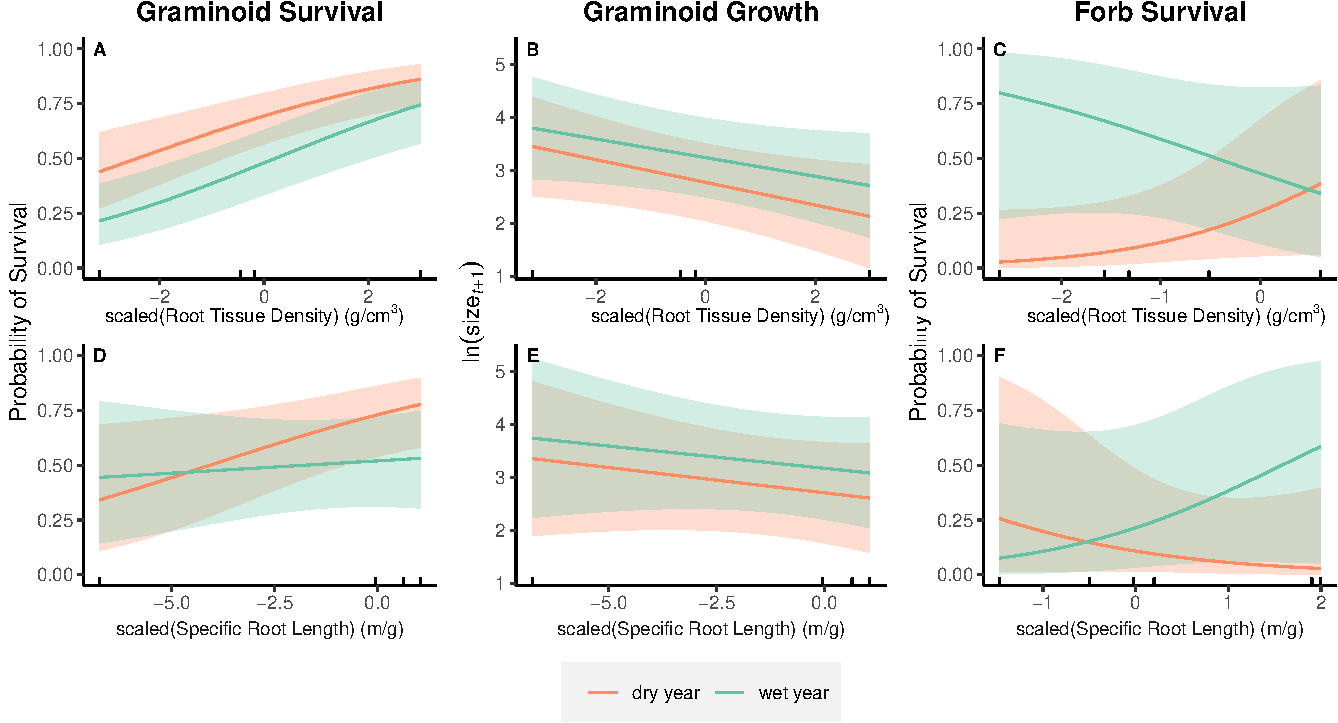
\includegraphics[width=.8\textwidth]{suppObservationsFig-1.pdf}
\caption{\small{
Illustration of the interaction between trait and SPEI for forb survival and graminoid survival and growth models for root tissue density and specific root length. These interactions were not significant. 
}}
\label{fig:GramSurv_all}
\end{figure}



\end{document}